\section{Top performers} % 3.4 Top performers
\urgent[inline]{List other top-selling games in the same market. Provide sales figures, release dates, information on sequels and platforms, as well as brief descriptions of each title.}

% \subsubsection{Ultimate Chicken Horse}

% La descripción de este videojuego se ha realizado ya en §\ref{subsubsec:UCH}, así
% que no se procederá a no repetir información.

% \textbf{Características destacadas:}
% \begin{itemize}
%     \item Multijugador online y local hasta 4 jugadores.
%     \item Dinámica de juego única que fomenta la competición.
%     \item Complejo si se desea usar estrategia, simple si no.
%     \item Distintos modos de juego.
% \end{itemize}

% \textbf{Limitaciones:}
% \begin{itemize}
%     \item A pesar de ser un juego festivo, también es un juego que tiende a
%     hacerse lento.
%     \item Los niveles a escoger son estáticos.
%     \item Los distintos personajes no tienen mecánica que los diferencien de los
%     demás, lo único diferente es la estética.
%     \item El juego no pertenece al género de acción, lo cual también se puede
%     observar en la velocidad de movimiento de los personajes.
% \end{itemize}

% \subsubsection{Jackbox Party Packs}
% % Nombre
% % Desarrollador + Editor
% % Año de publicación
% \emph{Jackbox Party Packs}, desarrollados y publicados por \emph{Jackbox Games,
% Inc.} desde el 2014, son una serie de videojuegos cada uno compuesto por una
% serie de minijuegos distintos que se pueden jugar online sin necesidad de que
% todos los participantes hayan comprado el juego.

% % Página web
% \url{https://www.jackboxgames.com/}

% \textbf{Capturas:}
% \begin{figure}[H]
%     \centering
%     \begin{minipage}{0.40\textwidth}
%         \centering
%         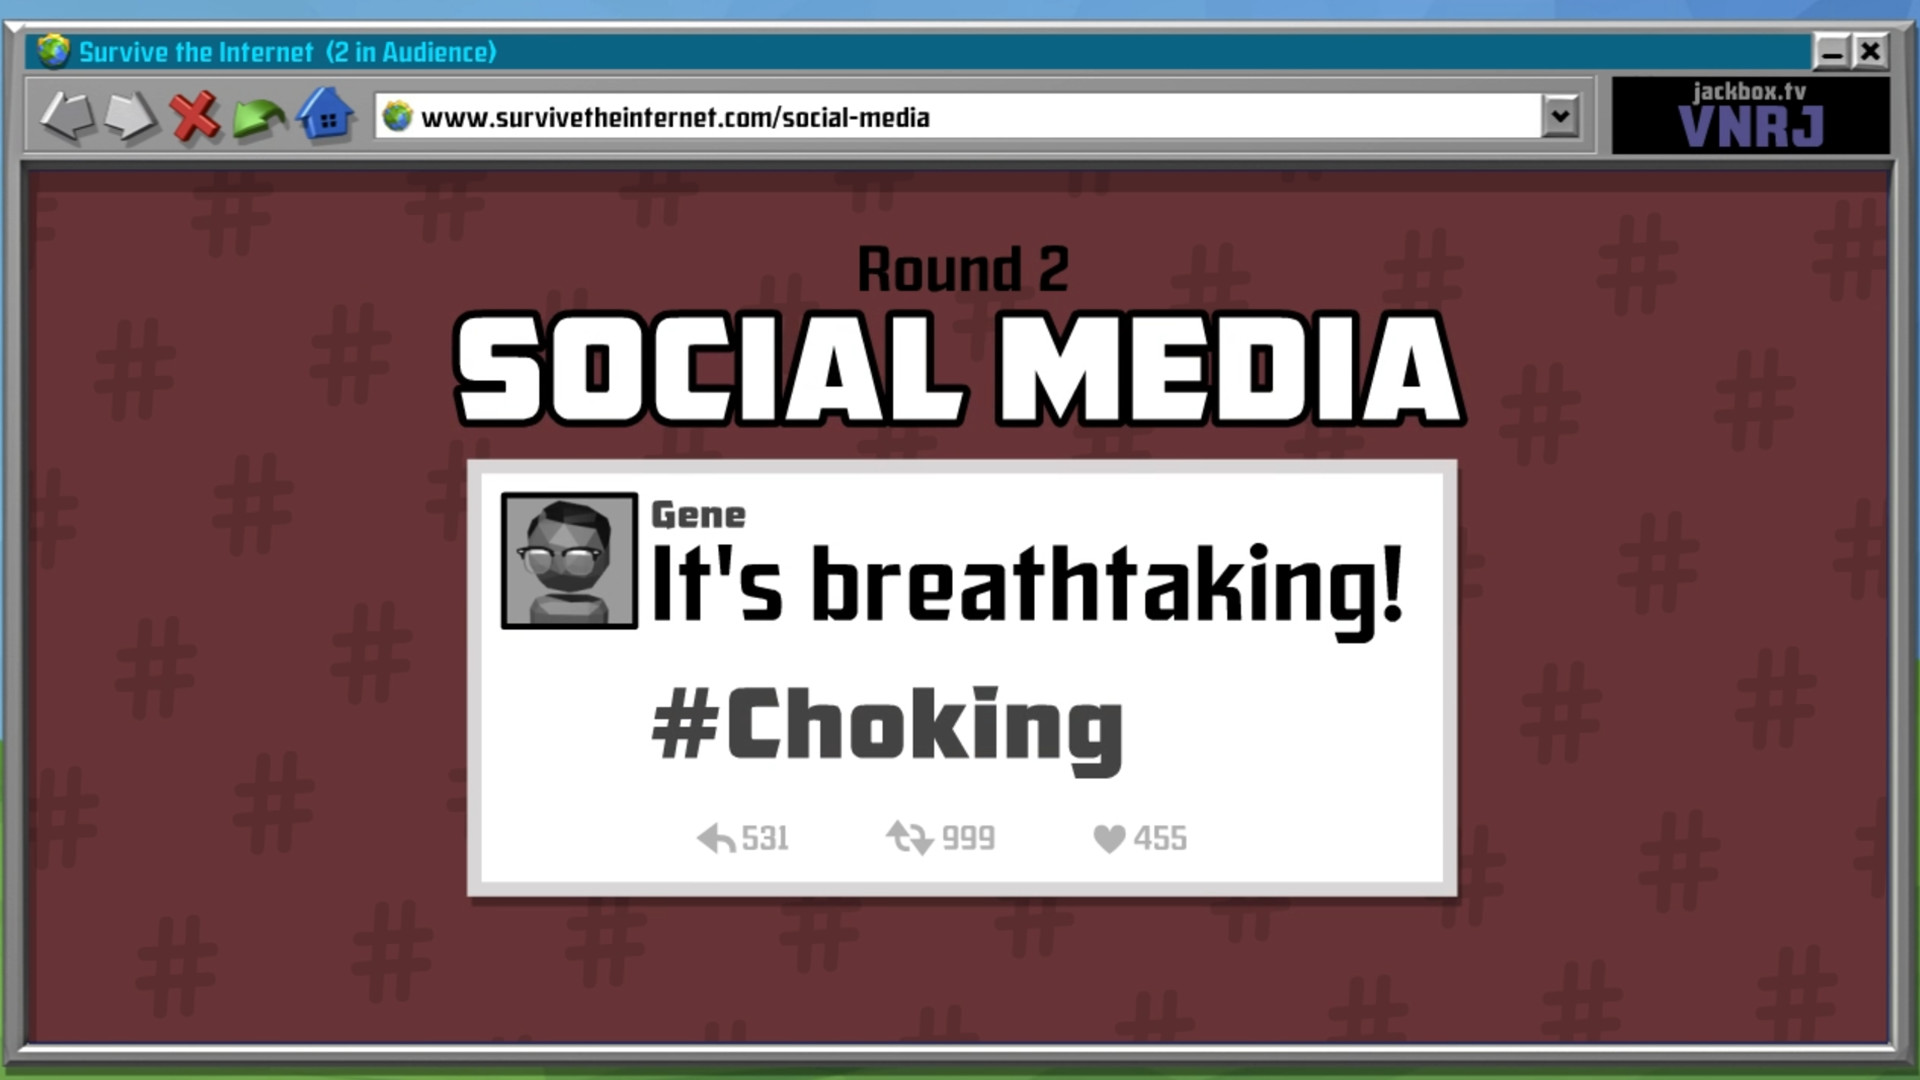
\includegraphics[width=1.0\textwidth]{Cuerpo/4/JPP1.jpg} %
%         \subcaption{Un minijuego de uno de los packs}
%         \label{JPP-Internet}
%     \end{minipage}\hfill
%     \begin{minipage}{0.40\textwidth}
%         \centering
%         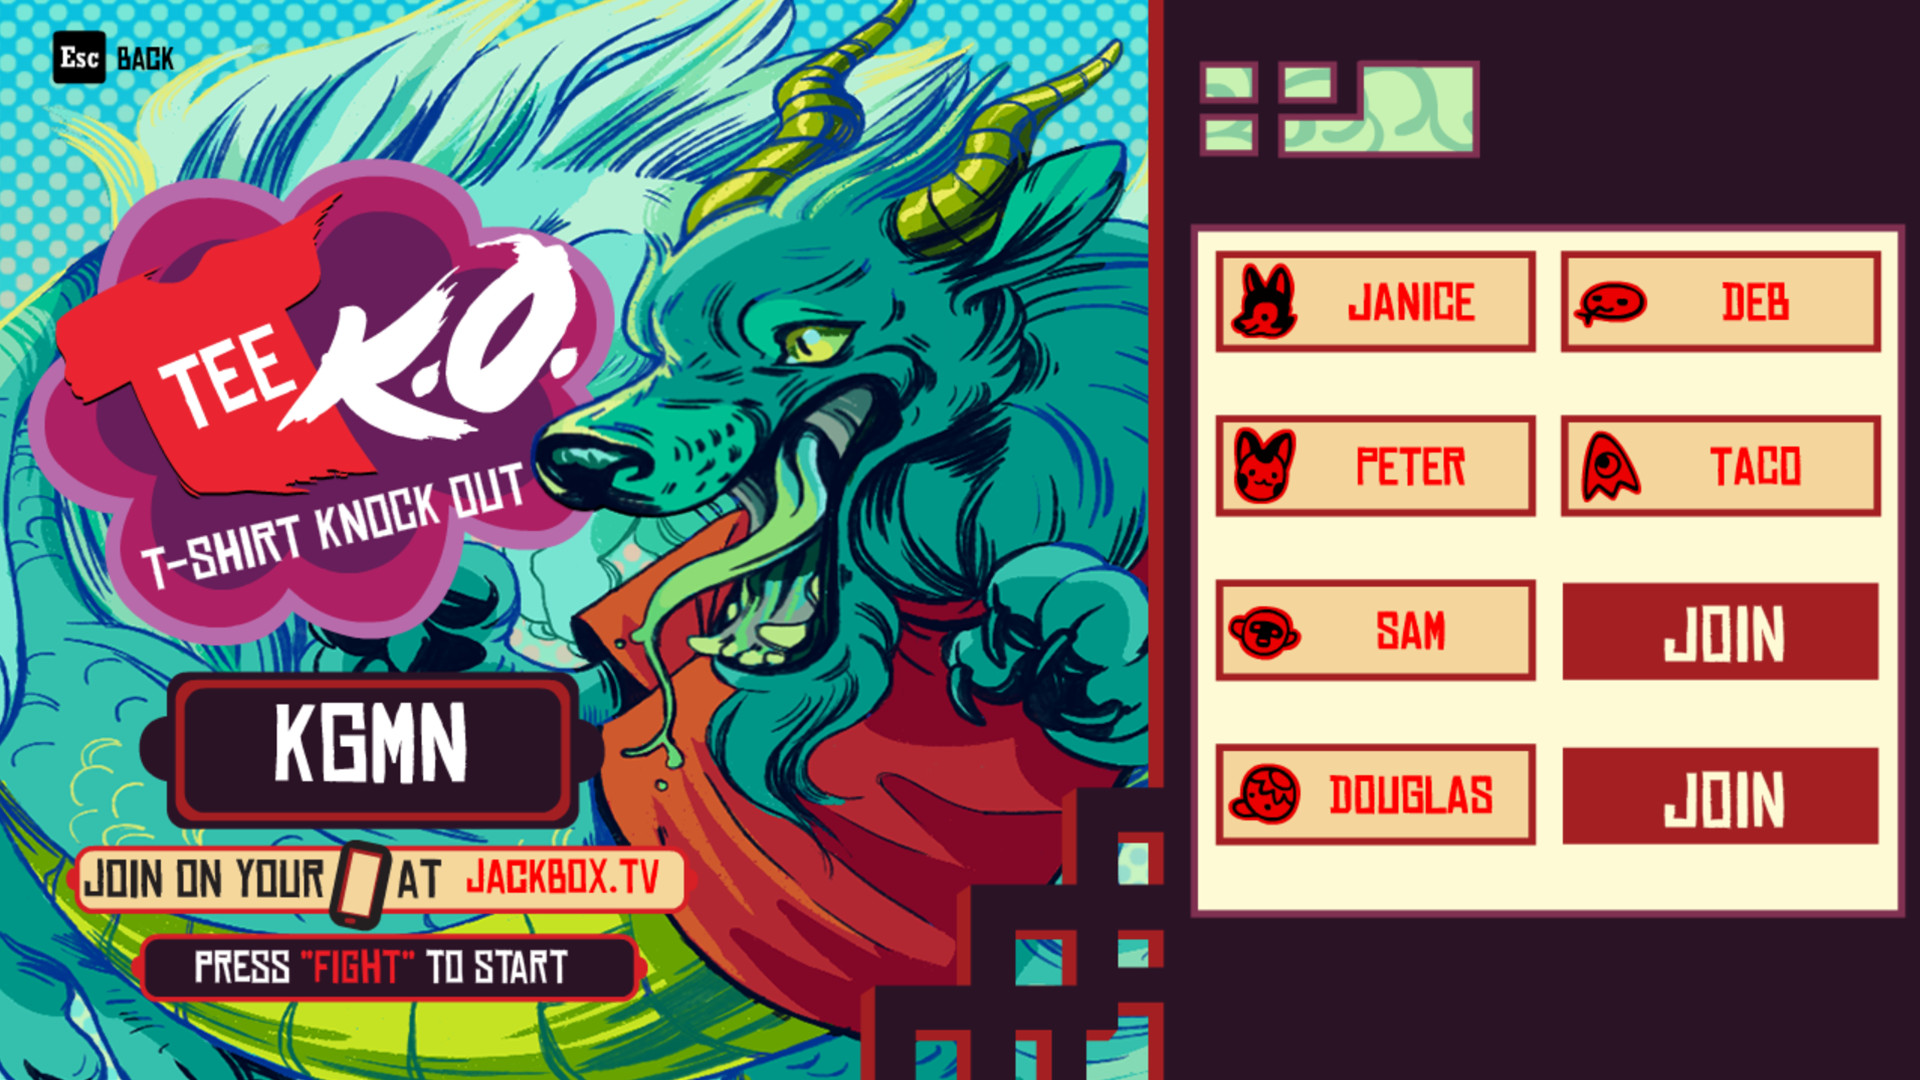
\includegraphics[width=1.0\textwidth]{Cuerpo/4/JPP2.jpg} %
%         \subcaption{Pantalla de inicio de otro minijuego}
%         \label{JPP-Inicio}
%     \end{minipage}
%     \centering
%     \begin{minipage}{0.40\textwidth}
%         \centering
%         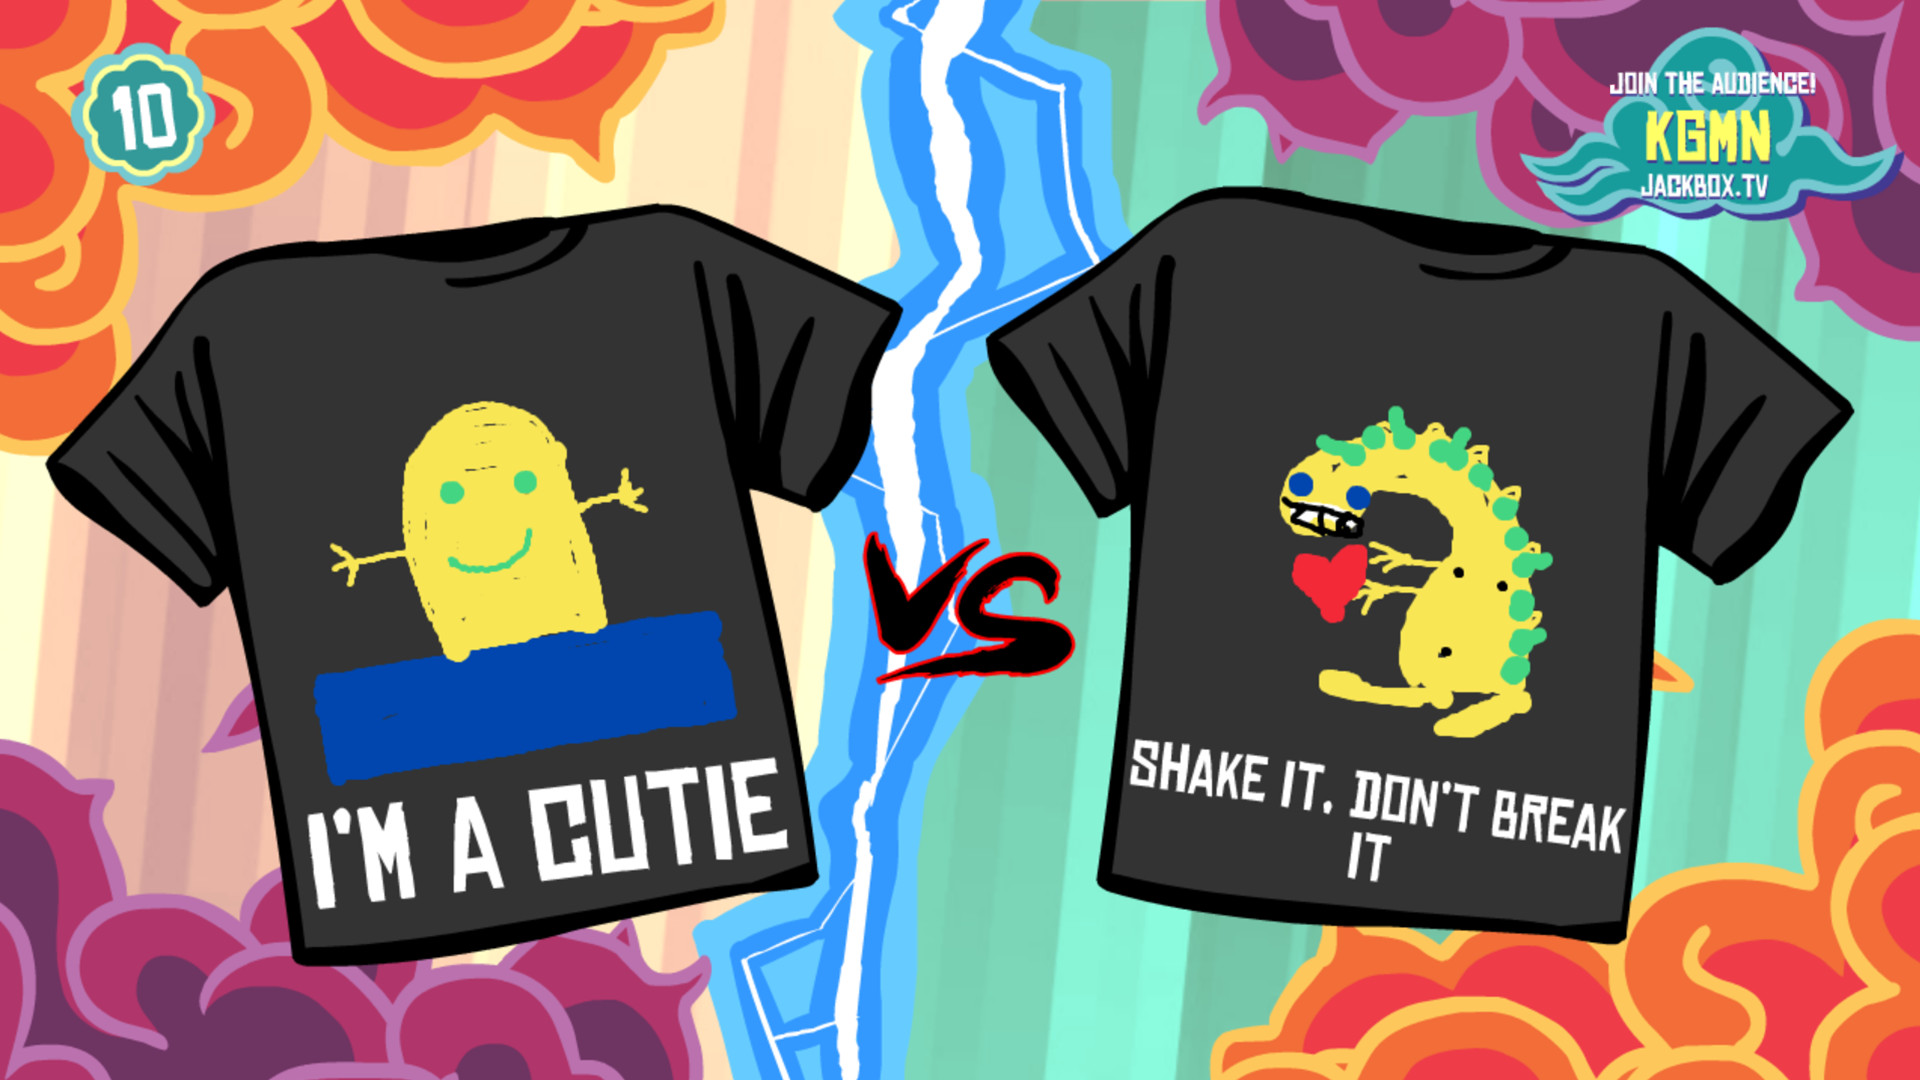
\includegraphics[width=1.0\textwidth]{Cuerpo/4/JPP3.jpg} %
%         \subcaption{Otro minijuego de uno de los packs}
%         \label{JPP-Tees}
%     \end{minipage}
%     \caption{Capturas de varios juegos de los Jackbox Party Packs}
% \end{figure}

% \textbf{Características destacadas:}
% \begin{itemize}
%     \item Tiene una multitud de minijuegos distintos.
%     \item Se caracteriza por tener una velocidad de juego relativamente rápida y
%     una partidas cortas.
%     \item Sólo una persona debe comprar el juego para que varias personas puedan
%     disfrutar del videojuego.
% \end{itemize}

% \textbf{Limitaciones:}
% \begin{itemize}
%     \item El hecho de que el paquete consista de múltiples minijuegos hace que
%     algunos no sean divertidos. Hay demasiada cantidad y poca calidad en
%     general.
%     \item El juego sólo está disponible en inglés.
%     \item Hay que comprar distintas versiones del juego para poder acceder a
%     distintos minijuegos.
% \end{itemize}

% \subsubsection{Pummel Party}
% % Nombre % Desarrollador + Editor % Año de publicación
% \emph{Pummel Party}, desarrollado y publicado por \emph{Rebuilt Games} en el
% 2018, es un juego festivo multijugador usando en la que se destruye a tus
% compañeros con una variedad de objetos y se compite por puntos en una colección
% de minijuegos distintos.

% La página oficial es: % Página web
% \url{http://www.rebuiltgames.com/}

% \textbf{Capturas:}
% \begin{figure}[H]
%     \centering
%     \begin{minipage}{0.40\textwidth}
%         \centering
%         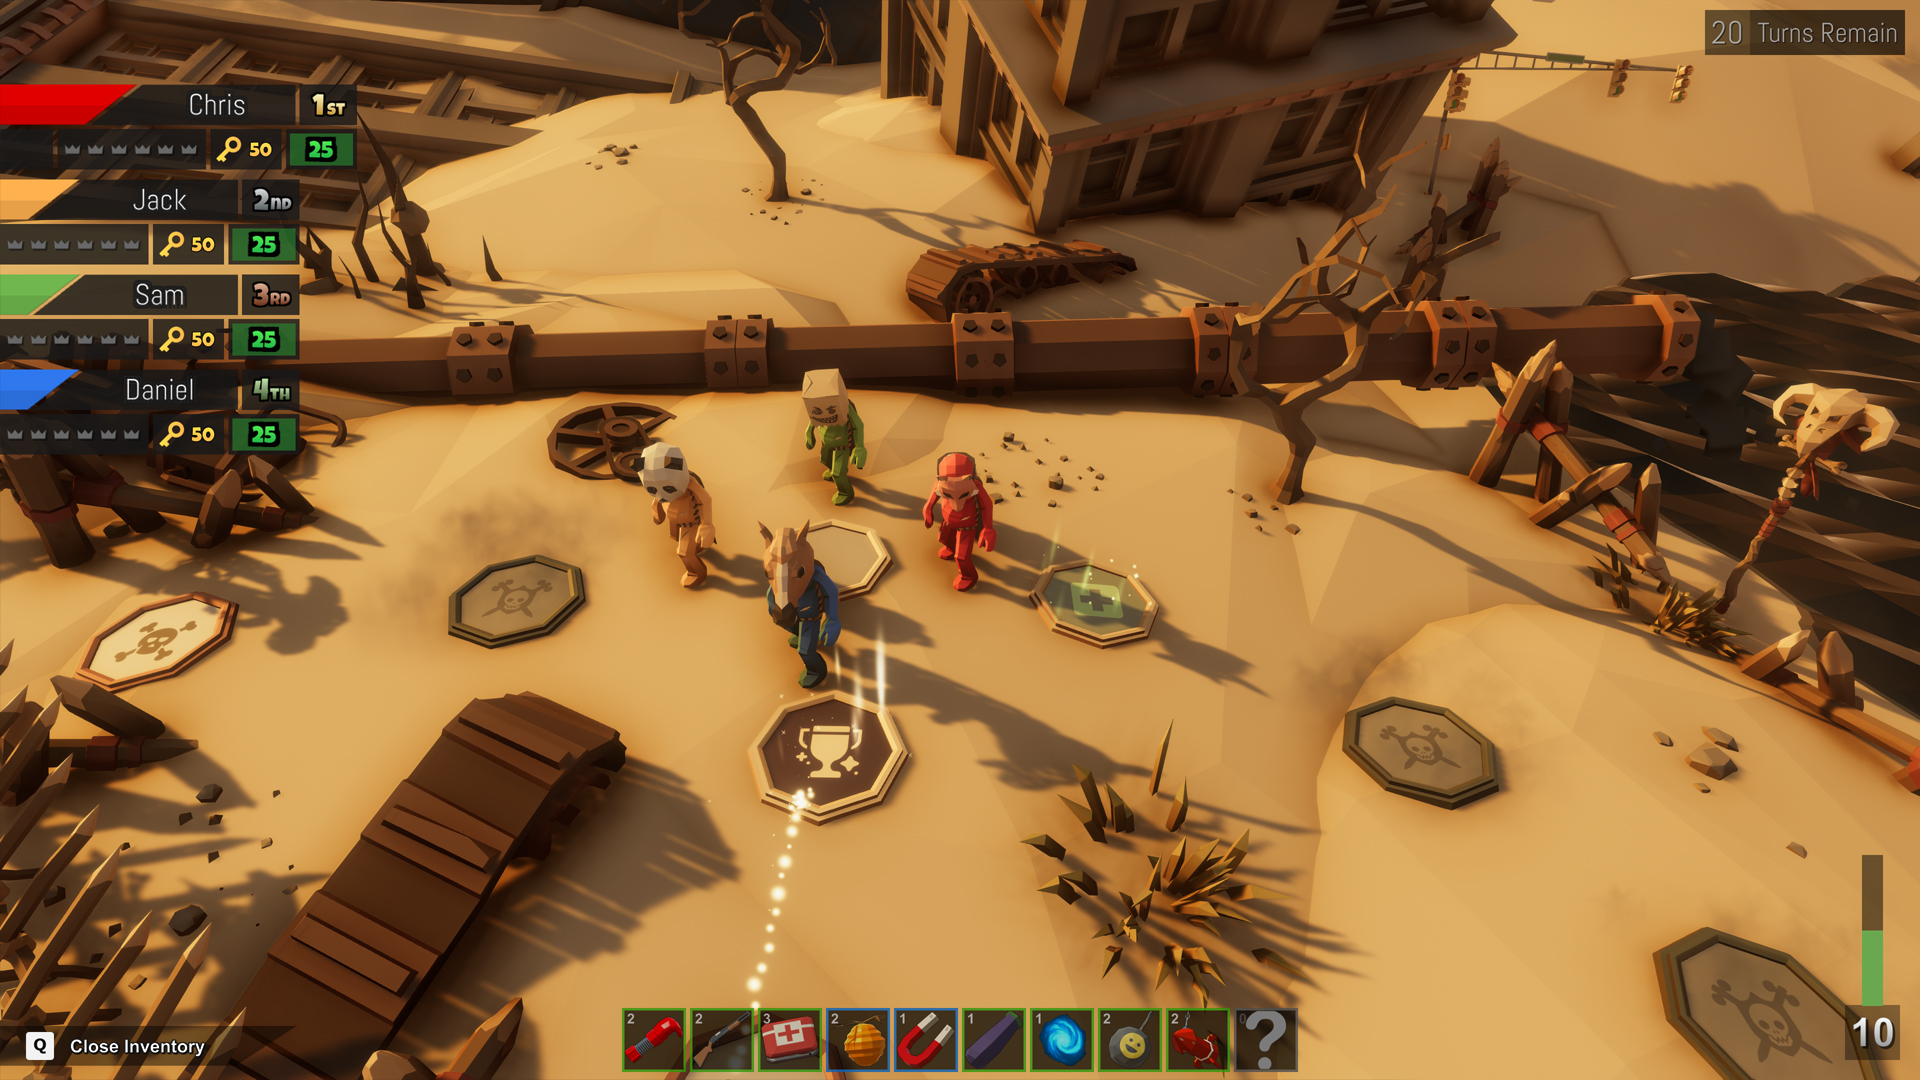
\includegraphics[width=1.0\textwidth]{Cuerpo/4/PMP1.jpg} %
%         \subcaption{El modo tablero de Pummel Party}
%         \label{PMP-Tablero}
%     \end{minipage}\hfill
%     \begin{minipage}{0.40\textwidth}
%         \centering
%         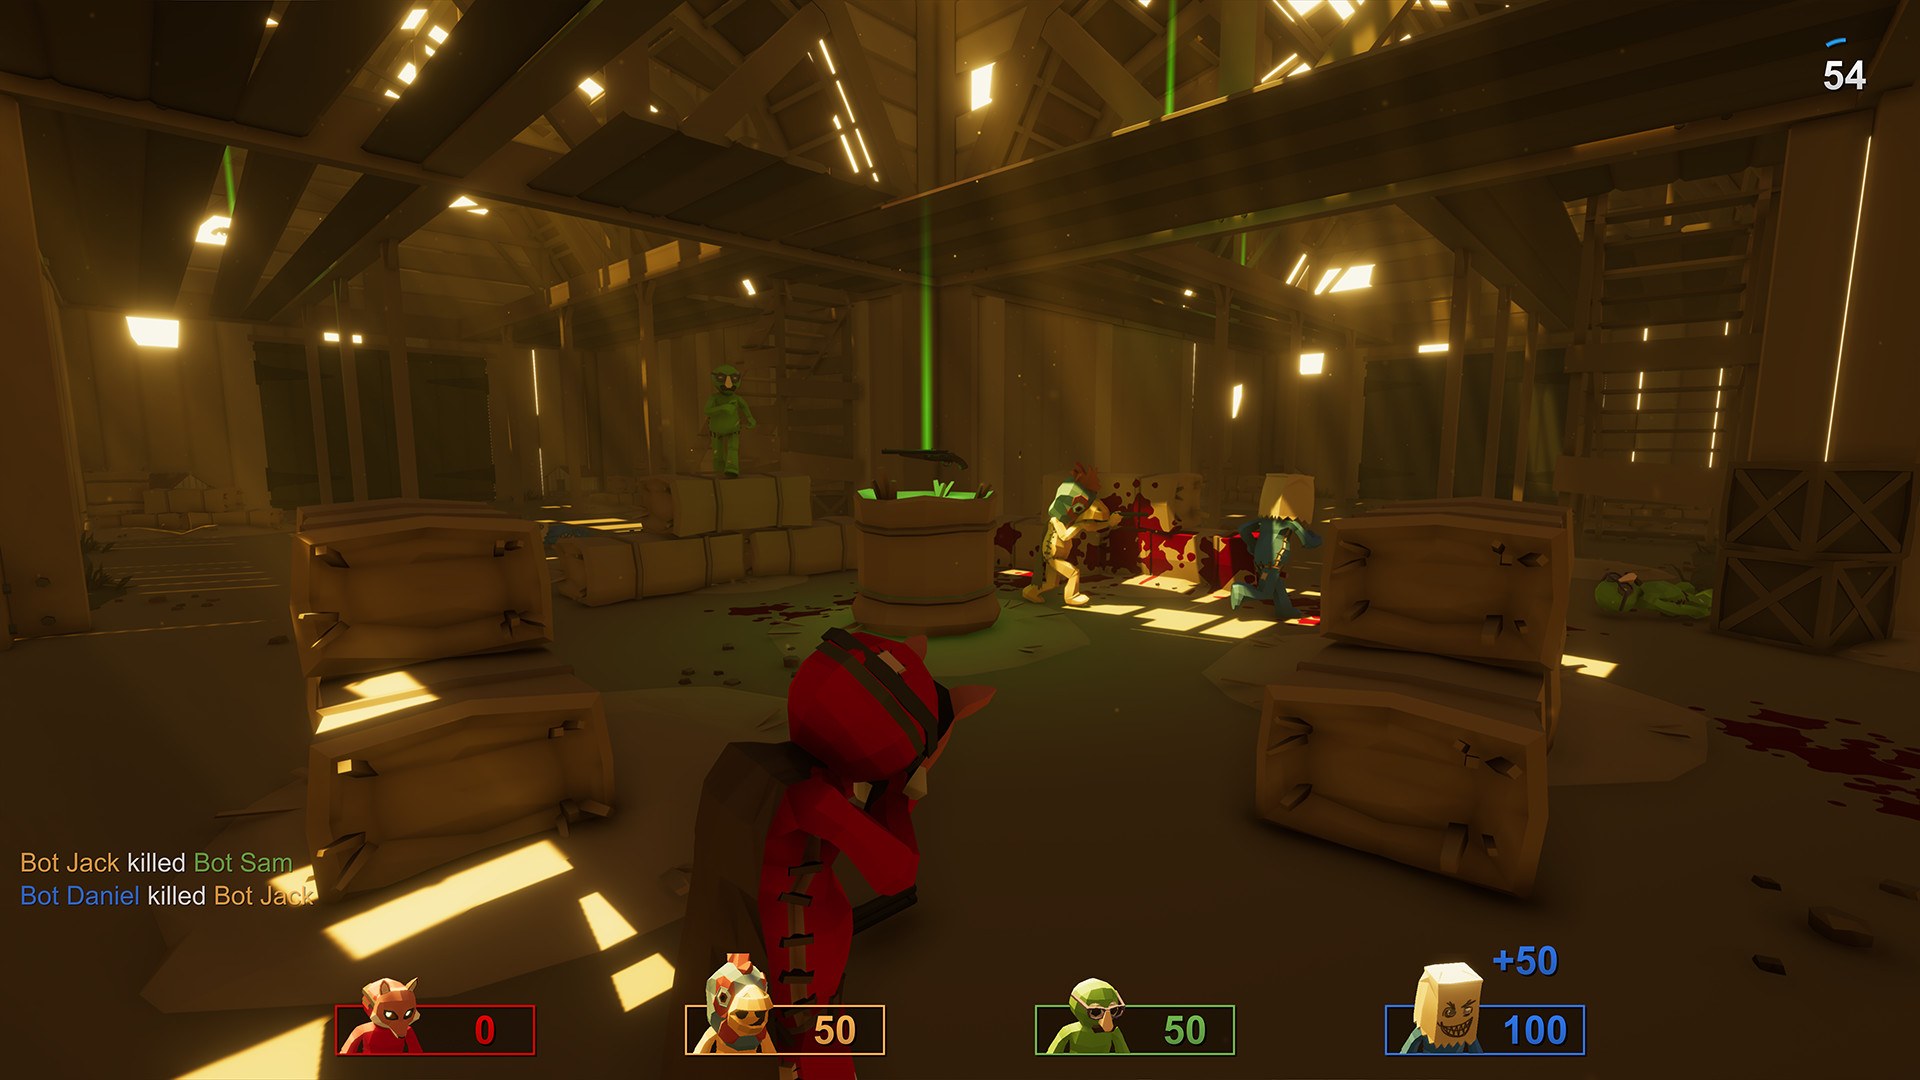
\includegraphics[width=1.0\textwidth]{Cuerpo/4/PMP2.jpg} %
%         \subcaption{Un minijuego de tipo shooter}
%         \label{PMP-Shooter}
%     \end{minipage}
%     \centering
%     \begin{minipage}{0.40\textwidth}
%         \centering
%         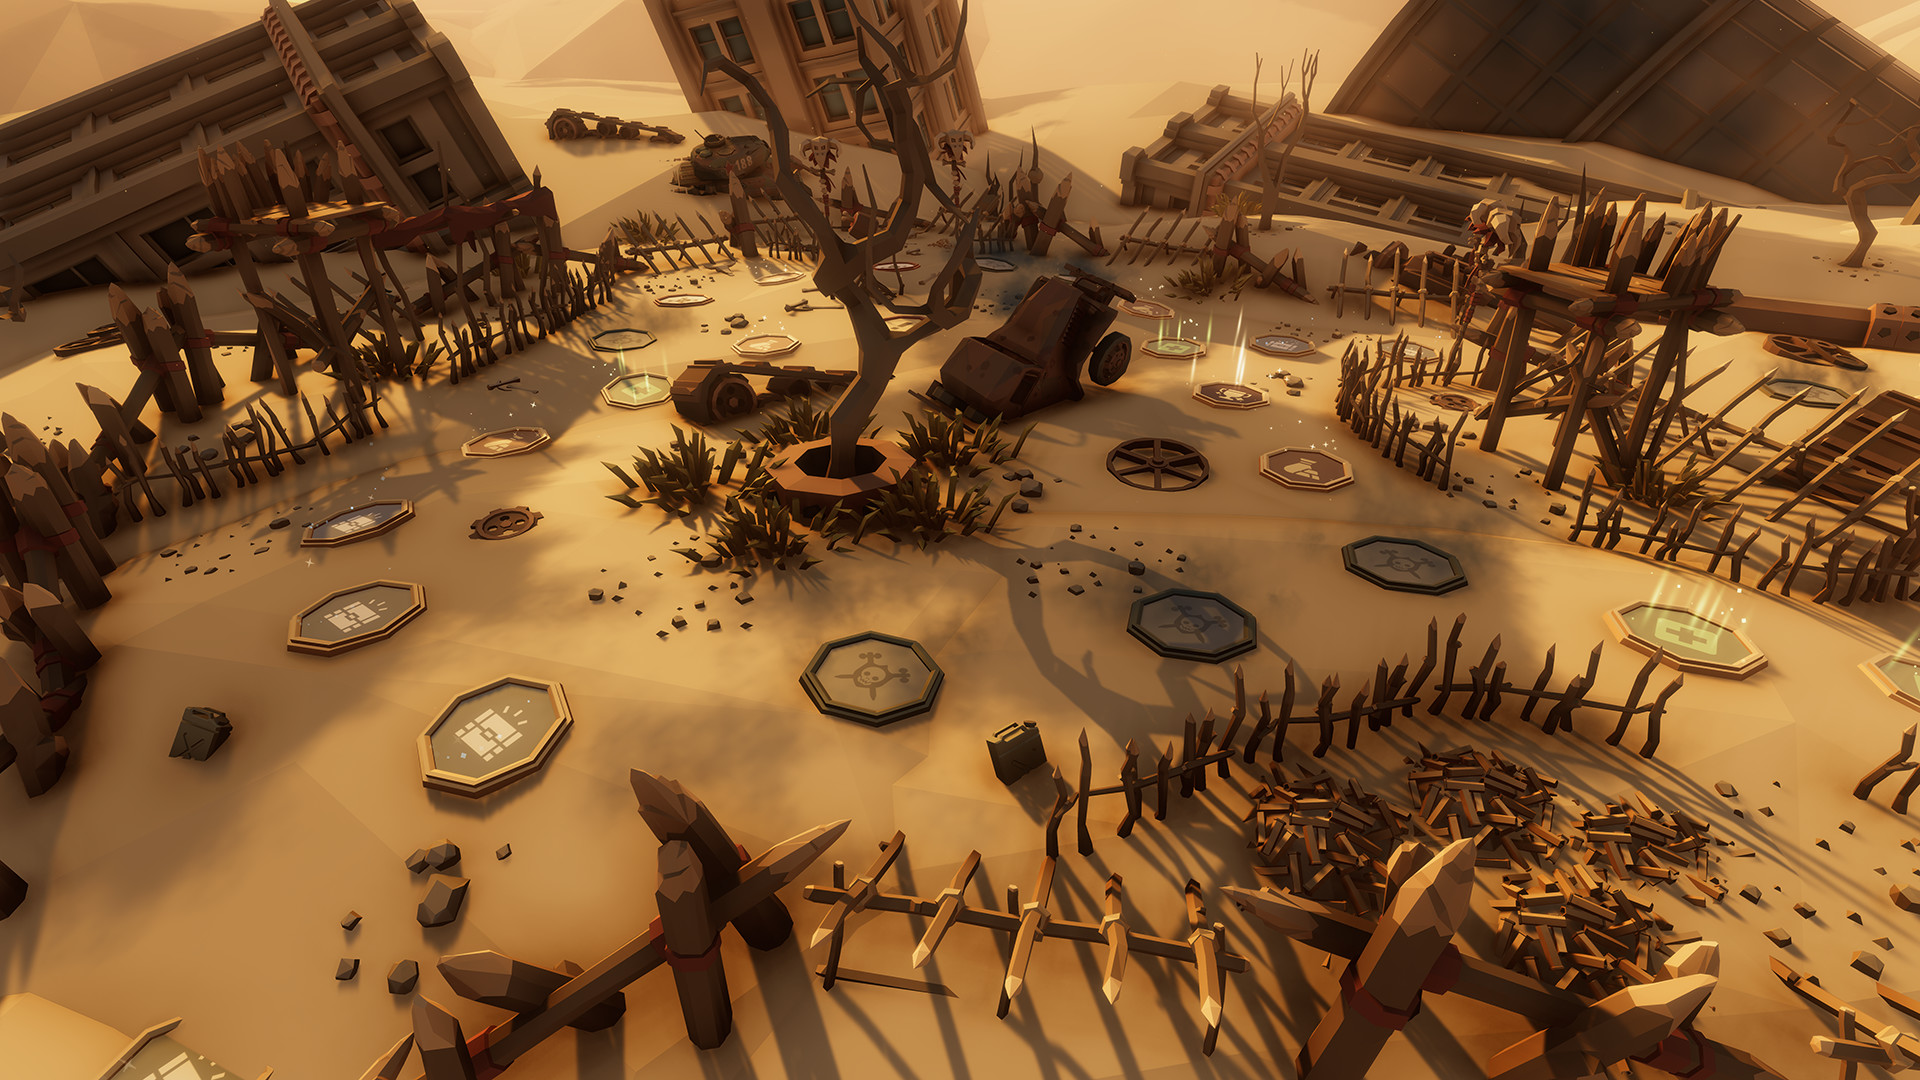
\includegraphics[width=1.0\textwidth]{Cuerpo/4/PMP3.jpg} %
%         \subcaption{Uno de los paisajes de un tablero}
%         \label{PMP-Paisaje}
%     \end{minipage}
%     \caption{Capturas de Pummel Party}
% \end{figure}

% \textbf{Características destacadas:}
% \begin{itemize}
%     \item Una gran cantidad de objetos para destruir a tus amigos.
%     \item Múltiples minijuegos distintos que fomentan la competitividad.
%     \item Traducido a múltiplos idiomas, incluido castellano.
% \end{itemize}

% \textbf{Limitaciones:}
% \begin{itemize}
%     \item El juego es por turnos, por lo cual hay que esperar a que cada jugador
%     tome una acción antes de poder avanzar.
%     \item Sufre de problemas de balance y una AI pobre.
%     \item Puede hacerse demasiado aleatorio y sin sentido a veces.
% \end{itemize}